\documentclass[main.tex]{subfiles}

\begin{document}

\section{Statica del corpo rigido}

\subsection{Fonti di studio}
Un ottimo canale youtube è ”Romaprof”, ricco di esercizi di statica risolti sia per metodo grafico che analitico, passo passo con spiegazioni.

\subsection{Gradi di libertà}
Un corpo rigido possiede, nel piano, 3 gradi di libertà, 2 traslazionali e uno rotazionale, ovvero può muoversi in 3 direzioni (in orizzontale, verticale e ruotare). Nello spazio, un corpo rigido possiede 6 gradi di libertà, 3 traslazionali e 3 rotazionali. In questo corso presteremo attenzione unicamente al caso piano.

\subsection{Asta nel piano}
Un’asta (figura \ref{asta_piano}), nel piano, viene rappresentata con una linea che viene chiamata asse baricentrico della trave (o asta).

\begin{figure}[H]
  \centering
  \resizebox{0.5\textwidth}{!}{\input{chapters/1/asta.tex}}
  \caption{Asta nel piano.}
  \label{asta_piano}
\end{figure}

\subsection{Vincoli}
Un vincolo è un oggetto che viene applicato ad un corpo rigido e ne va a limitare il moto. Esistono diverse tipologie di vincoli, ed ogni vincolo possiede caratteristiche particolari.

\subsubsection{Carrello}
Vincolo semplice che impedise un moto perpendicolare ad esso, cioè un modo che farebbe "staccare" il carrello dalla parete. In questa dispensa sarà indicato con il simbolo in figura \ref{carrello}. Questo vincolo impone 1 grado di vincolo.

\begin{figure}[H]
  \begin{subfigure}[b]{.5\textwidth}
  	\centering
  	\resizebox{0.5\textwidth}{!}{% First image 2015 06 29

\begin{tikzpicture}

  \tiny

  \point{a}{0}{0};
  \point{b}{5}{0};

  \support{2}{a};
  \beam{2}{a}{b};

  \notation{1}{a}{A}[above left];
  \notation{1}{b}{B}[above right];

\end{tikzpicture}}
  	\caption{Un carrello applicato ad un’asta.}
  \end{subfigure}
  \hfill
  \begin{subfigure}[b]{.5\textwidth}
  \centering
  	\resizebox{0.5\textwidth}{!}{\input{chapters/1/reazione_carrello.tex}}
  	\caption{La reazione vincolare di un carrello.}
  \end{subfigure}
  \caption{Il vincolo Carrello.}
  \label{carrello}
\end{figure}

\subsubsection{Pendolo semplice o Biella}
Vincolo semplice (figura \ref{biella}) che si oppone ad un moto lungo la propria direzione assiale. Questo vincolo impone 1 grado di vincolo.

\begin{figure}[H]
  \begin{subfigure}[b]{.5\textwidth}
  	\centering
  	\resizebox{0.5\textwidth}{!}{% First image 2015 06 29

\begin{tikzpicture}

  \tiny

  \point{a}{0}{0};
  \point{b}{5}{0};
  \point{c}{-1}{-1}

  %\load{1}{a}[90];
  \beam{2}{a}{b};
  \beam{2}{c}{a};

  \hinge{1}{a}
  \hinge{1}{c}

  \support{1}{c}

  \notation{1}{a}{A}[above left];
  \notation{1}{b}{B}[above right];

\end{tikzpicture}}
  	\caption{Un pendolo applicato ad un’asta.}
  \end{subfigure}
  \hfill
  \begin{subfigure}[b]{.5\textwidth}
  \centering
  	\resizebox{0.5\textwidth}{!}{% First image 2015 06 29

\begin{tikzpicture}

  \tiny

  \point{a}{0}{0};
  \point{b}{5}{0};
  \point{c}{-1}{-1}

  \load{1}{a}[-135];
  \beam{2}{a}{b};

  \notation{1}{a}{A}[above left];
  \notation{1}{b}{B}[above right];

\end{tikzpicture}}
  	\caption{La reazione vincolare di un pendolo.}
  \end{subfigure}
  \caption{Il vincolo Pendolo.}
  \label{biella}
\end{figure}

\subsubsection{Cerniera}
Vincolo doppio (figura \ref{cerniera}) che consente unicamente la rotazione, quando è bloccato a terra, o blocca i movimenti assiali delle aste quando interna.

\begin{figure}[H]
  \begin{subfigure}[b]{.5\textwidth}
  	\centering
  	\resizebox{0.5\textwidth}{!}{% First image 2015 06 29

\begin{tikzpicture}

  \tiny

  \point{a}{0}{0};
  \point{b}{5}{0};

  %\load{1}{a}[90];
  \beam{2}{a}{b};

  \hinge{1}{a}
  \support{1}{a}

  \notation{1}{a}{A}[above left];
  \notation{1}{b}{B}[above right];

\end{tikzpicture}}
  	\caption{Una cerniera ancorata applicata ad un’asta impone $2 gdv$.}
  \end{subfigure}
  \hfill
  \begin{subfigure}[b]{.5\textwidth}
  \centering
  	\resizebox{0.5\textwidth}{!}{% First image 2015 06 29

\begin{tikzpicture}

  \tiny

  \point{a}{0}{0};
  \point{b}{2}{0};
  \point{c}{4}{0};
  \point{d}{2}{2};

  %\load{1}{a}[90];
  \beam{2}{a}{b};
  \beam{2}{b}{c};
  \beam{2}{d}{b};

  \hinge{1}{b}

  \notation{1}{a}{A}[above left];
  \notation{1}{b}{B}[below=0.2];
  \notation{1}{d}{D}[above];
  \notation{1}{c}{C}[above right];

\end{tikzpicture}}
  	\caption{Una cerniera interna applicata a 3 aste impone $2(3 - 1) = 4gdv$.}
  \end{subfigure}
  \caption{Il vincolo Cerniera.}
  \label{cerniera}
\end{figure}

\subsubsection{Incastro}
Vincolo triplo (figura \ref{incastro}) che impedisce qualsiasi movimento quando applicato ad un corpo rigido.

\begin{figure}[H]
  \begin{subfigure}[b]{.5\textwidth}
  	\centering
  	\resizebox{0.5\textwidth}{!}{% First image 2015 06 29

\begin{tikzpicture}

  \tiny

  \point{a}{0}{0};
  \point{b}{5}{0};

  %\load{1}{a}[90];
  \beam{2}{a}{b};

  \support{3}{a}[-90]

  \notation{1}{a}{A}[above right];
  \notation{1}{b}{B}[above right];

\end{tikzpicture}}
  	\caption{Un incastro applicato ad un’asta impone $3 gdv$.}
  \end{subfigure}
  \hfill
  \begin{subfigure}[b]{.5\textwidth}
  \centering
  	\resizebox{0.5\textwidth}{!}{% First image 2015 06 29

\begin{tikzpicture}

  \tiny

  \point{a}{0}{0};
  \point{b}{5}{0};

  %\load{1}{a}[90];
  \beam{2}{a}{b};

  \load{1}{a}[90]
  \load{1}{a}[180]
  \load{3}{a}

  \notation{1}{a}{A}[above left];
  \notation{1}{b}{B}[above right];

\end{tikzpicture}}
  	\caption{Le reazioni vincolari di un incastro.}
  \end{subfigure}
  \caption{Il vincolo Incastro.}
  \label{incastro}
\end{figure}

\subsection{L'analisi (o computo) dei vincoli}
Per computo dei vincoli si intende contare tutti i gradi di libertà e di vincolo di un sistema di corpi rigidi e vincoli per dare una prima approssimazione alla categoria in cui questo sistema va ad appartenere. Si tratta di una approssimazione perché esistono casi particolari in cui questa fallisce, che sono illustrati alla fine di questa sotto sezione. È importante tenere a mente il teorema delle cerniere interne mentre si procede con il calcolo.

\subsubsection{Struttura Isostatica: $gdv = gdl$}
Le strutture isostatiche son oggetto di questo corso. Il calcolo delle reazioni interne in questi sistemi è sempre risolubile tramite un sistema lineare.

\subsubsection{Struttura Iperstatica: $gdv > gdl$}
Viene chiamato livello di iperstaticità della struttura $i$ il delta tra $gdv$ e $gdl$ ed indica il numero di incognite agguntive che vengono introdotte per risolvere il sistema delle reazioni interne.

\subsubsection{Struttura Labile: $gdv < gdl$}
Una struttura che potrebbe essere mossa da una forza esterna.

\subsection{Limiti del computo dei vincoli}

\subsubsection{Esempio 1}
Struttura (figura \ref{es1}) apparentemente iperstatica ma con vincoli a carrello con e senza cerniera ”ridondanti”, per cui risulta labile.

\begin{figure}[H]
  \centering
  \resizebox{0.75\textwidth}{!}{% First image 2015 06 29

\begin{tikzpicture}

  \tiny

  \point{a}{0}{0};
  \point{b}{1}{0};
  \point{c}{2}{0};
  \point{d}{3}{0};
  \point{e}{4}{0};
  \point{f}{5}{0};
  \point{g}{6}{0};
  \point{h}{7}{0};

  \support{2}{a}
  \support{2}{b}
  \support{2}{c}
  \support{2}{d}
  \support{2}{e}
  \support{2}{f}
  \support{2}{g}
  \support{2}{h}

  \hinge{2}{b}[a][h][2]
  \hinge{2}{c}[a][h][2]
  \hinge{2}{d}[a][h][2]
  \hinge{2}{e}[a][h][2]
  \hinge{2}{f}[a][h][2]
  \hinge{2}{g}[a][h][2]

  \beam{2}{a}{h}

  \load{1}{d}[45]

\end{tikzpicture}}
  \caption{Esempio 1: Struttura apparentemente \textit{iperstatica}.}
  \label{es1}
\end{figure}

\subsubsection{Esempio 2}
Struttura (figura \ref{es2}) che al calcolo dei vincoli risulta isostatica, potrebbe sembrare labile in base all’esempio precedente, ma che in seguito all’applicazione di un’unica forza verticale risulta addirittura iperstatica.

\begin{figure}[H]
  \centering
  \resizebox{0.75\textwidth}{!}{% First image 2015 06 29

\begin{tikzpicture}

  \tiny

  \point{a}{0}{0};
  \point{b}{2}{0};
  \point{c}{4}{0};

  \support{2}{a}
  \support{2}{b}
  \support{2}{c}

  \hinge{2}{b}[a][c][2]

  \beam{2}{a}{c}

  \load{1}{b}[90]

\end{tikzpicture}}
  \caption{ Esempio 1: Struttura apparentemente \textit{iperstatica}.}
  \label{es2}
\end{figure}

\subsection{Caratteristiche della sollecitazione interna}
Immaginiamo di tagliare un’asta (figura \ref{sollecitazione_interne}) in un punto S1, ottenendo così due tronchi, $t1$ e $t2$. In quel punto agiscono un \textbf{taglio} T verticale, una \textbf{forza normale} N ed un \textbf{momento flettente} M.

\begin{figure}[H]
  \centering
  \resizebox{0.75\textwidth}{!}{\begin{tikzpicture}

  \tiny

  \point{a}{0}{0};
  \point{b}{2}{0};
  \point{c}{4}{0};
  \point{d}{6}{0};
  \point{e}{8}{0};

  \notation{5}{a}{b}[$t_1$][.5][above][1];
  \notation{5}{d}{e}[$t_2$][.5][above][1];
  \notation{1}{c}{$S_1$}[above];

  \beam{2}{a}{b};
  \beam{2}{d}{e};

  \load{1}{b}
  \load{1}{b}[-90]
  \load{3}{b}

  \load{1}{d}[180]
  \load{1}{d}[90]
  \load{2}{d}

\end{tikzpicture}}
  \caption{Le caratteristiche di sollecitazione interne nel punto S1.}
  \label{sollecitazione_interne}
\end{figure}

Se ora andiamo a fare un secondo taglio S2, punto definito come S2 = S1 + ds, costruiamo un segmento infinitesimo di tronco che viene chiamato concio elementare. In particolare, siccome noi stiamo guardando proiezioni sul piano di corpi rigidi, viene chiamato sezione laterale di concio elementare, che è da ambo i lati soggetto alle sollecitazioni interne dell’asta.

\begin{figure}[H]
  \centering
  \resizebox{0.5\textwidth}{!}{\begin{tikzpicture}

  \tiny

  \point{a}{0}{0};
  \point{b}{0}{1};
  \point{c}{1}{1};
  \point{d}{1}{0};

  \point{z}{0.5}{0.5}

  \point{m}{-0.25}{0.5}
  \point{n}{1.25}{0.5}


  \beam{2}{a}{b}[0][1]
  \beam{2}{b}{c}[0][1]
  \beam{2}{c}{d}[0][1]
  \beam{2}{d}{a}[0][1]

  \load{1}{m}[180]
  \load{1}{m}[90]
  \load{2}{m}[90][180]

  \load{1}{n}
  \load{1}{n}[-90]
  \load{3}{n}[-90][180]

  %\notation{6}{z}{+};


\end{tikzpicture}}
  \caption{Sezione di concio elementare.}
\end{figure}

\subsubsection{Convenzione per lo sforzo normale baricentrico}
Viene considerato positivo quando esso impone una trazione (figura \ref{normale_positivo}), mentre viene considerato negativo se esso impone una contrazione (figura \ref{normale_negativo}).

\begin{figure}[H]
  \begin{subfigure}[b]{.5\textwidth}
  	\centering
  	\resizebox{0.5\textwidth}{!}{\begin{tikzpicture}

  \tiny

  \point{a}{0}{0};
  \point{b}{0}{1};
  \point{c}{1}{1};
  \point{d}{1}{0};

  \point{z}{0.5}{0.5}

  \point{h}{0.5}{1}
  \point{w}{0.5}{0}

  \point{m}{0}{0.5}
  \point{n}{1}{0.5}

  \point{m1}{-1.25}{0.5}
  \point{n1}{2.25}{0.5}

  \beam{2}{a}{b}[0][1]
  \beam{2}{b}{c}[0][1]
  \beam{2}{c}{d}[0][1]
  \beam{2}{d}{a}[0][1]

  \load{1}{m1}

  \load{1}{n1}[180]

  \notation{6}{z}{+};


\end{tikzpicture}}
  	\caption{Sforzo normale di \textit{trazione}, positivo.}
  	\label{normale_positivo}
  \end{subfigure}
  \hfill
  \begin{subfigure}[b]{.5\textwidth}
  \centering
  	\resizebox{0.5\textwidth}{!}{\input{chapters/1/normale_negativo.tex}}
  	\caption{Sforzo normale di \textit{compressione}, negativo.}
  	\label{normale_negativo}
  \end{subfigure}
  \caption{Convenzione dello sforzo normale baricentrico.}
\end{figure}

\subsubsection{Convenzione per il taglio}
Viene considerato positivo quando esso impone al concio una rotazione oraria (figura \ref{taglio_positivo}), cioè a sinistra del concio il taglio va verso l’alto e a destra verso il basso, mentre è negativo quando esso impone al concio una rotazione anti-oraria (figura \ref{taglio_negativo}), cioè a sinistra del concio il taglio va verso il basso e a destra verso l’alto.

\begin{figure}[H]
  \begin{subfigure}[b]{.5\textwidth}
    \centering
    \resizebox{0.5\textwidth}{!}{\input{chapters/1/taglio_positivo.tex}}
    \caption{Taglio con \textit{rotazione oraria,}, positivo.}
    \label{taglio_positivo}
  \end{subfigure}
  \hfill
  \begin{subfigure}[b]{.5\textwidth}
  \centering
    \resizebox{0.5\textwidth}{!}{\input{chapters/1/taglio_negativo.tex}}
    \caption{Taglio con \textit{rotazione anti-oraria}, negativo.}
    \label{taglio_negativo}
  \end{subfigure}
  \caption{Convenzione del taglio.}
\end{figure}

\subsubsection{Convenzione per il momento flettente}
È considerato positivo (figura \ref{convenzione_momento}) quando tende le fibre inferiori ed è sempre disegnato dalla parte delle fibre tese.

\begin{figure}[H]
  \begin{subfigure}[b]{.5\textwidth}
    \centering
    \resizebox{0.5\textwidth}{!}{\begin{tikzpicture}

  \tiny

  \point{a}{0}{0};
  \point{b}{0}{1};
  \point{c}{1}{1};
  \point{d}{1}{0};

  \point{z}{0.5}{0.5}

  \point{h}{-0.5}{0.5}
  \point{w}{1.5}{0.5}

  \beam{2}{a}{b}[0][1]
  \beam{2}{b}{c}[0][1]
  \beam{2}{c}{d}[0][1]
  \beam{2}{d}{a}[0][1]

  \load{2}{h}[90][180]

  \load{3}{w}[-90][180]

  \internalforces{a}{b}{-0.25}{0};
  \internalforces{d}{c}{0.25}{0};

  \notation{6}{z}{-};


\end{tikzpicture}}
    \caption{Momento dalla parte delle fibre tese, positivo}
    \label{momento_positivo}
  \end{subfigure}
  \hfill
  \begin{subfigure}[b]{.5\textwidth}
  \centering
    \resizebox{0.5\textwidth}{!}{\input{chapters/1/momento_negativo.tex}}
    \caption{Momento dalla parte opposta alle fibre tese, negativo.}
    \label{momento_negativo}
  \end{subfigure}
  \caption{Convenzione del momento flettente.}
  \label{convenzione_momento}
\end{figure}

\subsection{Grafici della sollecitazione interna}
Si tratta di una serie di convenzioni adottate per comodità nel lavoro di chi fa studi di statica. Per comprendere al meglio come questi grafici vengono realizzati, guardate agli esercizi svolti più avanti nella dispensa.

\subsubsection{Convenzione grafica dello sforzo normale}
In alto positivo, in basso negativo. A destra positivo, a sinistra negativo.

\begin{figure}[H]
  \centering
  \resizebox{0.5\textwidth}{!}{\begin{tikzpicture}

  \tiny

  \point{a}{0}{0};
  \point{a1}{0.5}{0};
  \point{d}{0.5}{1/(sqrt(3)/2)}
  \point{d1}{0}{1/(sqrt(3)/2)}
  \point{b}{1}{2/(sqrt(3)/2)}
  \point{b1}{1.5}{2/(sqrt(3)/2)}

  \beam{2}{a}{b};

  \internalforces{a}{d}{-0.5}{-0.5}[0][red];
  \internalforces{d}{b}{0.5}{0.5}[0][blue];

\end{tikzpicture}}
  \caption{Convenzione grafica dello sforzo normale.}
\end{figure}

\subsubsection{Convenzione grafica del taglio}
In alto positivo, in basso negativo. A destra positivo, a sinistra negativo.

\begin{figure}[H]
  \centering
  \resizebox{0.5\textwidth}{!}{% First image 2015 06 29

\begin{tikzpicture}

  \tiny

  \point{a}{0}{0}
  \point{e}{2.5}{-0.866}
  \point{b}{0.5}{0.866}
  \point{d}{1.5}{0.866}
  \point{c}{1}{2*0.866}

  \beam{2}{a}{c}

  \internalforces{a}{b}{0.866}{0.866}[0][blue];
  \internalforces{b}{c}{-1.732}{-1.732}[0][red];

\end{tikzpicture}}
  \caption{Convenzione grafica del taglio.}
\end{figure}

\subsubsection{Convenzione grafica del momento flettente}
\textbf{Sempre dalla parte delle fibre tese}, cioè dalla parte dove le forze di taglio vanno a tirare le fibre dell'asta (nel disegno, nel caso della figura qui riportata, le fibre sono dalla parte inferiore), o alternativamente in alto negativo, in basso positivo. A destra negativo, a sinistra positivo.

\begin{figure}[H]
  \centering
  \resizebox{0.5\textwidth}{!}{% First image 2015 06 29

\begin{tikzpicture}

  \tiny

  \point{a}{0}{0}
  \point{e}{2.5}{-0.866}
  \point{b}{0.5}{0.866}
  \point{d}{1.5}{0.866}
  \point{c}{1}{2*0.866}

  \beam{2}{a}{c}

  \internalforces{a}{b}{0.5*1.732}{-1.732}[0][red];
  \internalforces{b}{c}{-1.732}{0}[0][red];

\end{tikzpicture}}
  \caption{Convenzione grafica del momento flettente.}
\end{figure}

\end{document}